\documentclass[../main.tex]{subfiles}
% Preamble
\begin{document}
	\chapter{DISE�O E IMPLEMENTACI�N DE LA APLICACI�N}
		\newpage
		
		\section{Casos de uso}
		Los Casos de Uso en Ingenier�a del software, es una t�cnica para la captura de requisitos potenciales de un nuevo Sistema o
		una actualizaci�n de Software. Cada caso de uso proporciona uno o m�s escenarios que indican c�mo deber�a interactuar el
		sistema con el usuario o con otro sistema para conseguir un objetivo espec�fico. Normalmente, en los casos de usos se evita
		el empleo de jergas t�cnicas, prefiriendo en su lugar un lenguaje m�s cercano al usuario final.
		
		En 1986, Ivar Jacobson, importante contribuyente al desarrollo de los modelos de UML y proceso unificado, cre� el concepto
		de caso de uso. 

		Durante los a�os 1990 los casos de uso se convirtieron en una de las pr�cticas m�s comunes para la captura de requisitos
		funcionales, especialmente con el desarrollo del paradigma de la programaci�n orientada a objetos, donde se originaron, si
		bien puede utilizarse con resultados igualmente satisfactorios con otros paradigmas de programaci�n.
		
		Un caso de uso es una secuencia de interacciones que se desarrollar�n entre un sistema y sus actores en respuesta a un evento
		que inicia un actor principal sobre el propio sistema. Los diagramas de casos de uso sirven para especificar la comunicaci�n
		y el comportamiento de un sistema mediante su interacci�n con los usuarios y/u otros sistemas. O lo que es igual, un diagrama
		que muestra la relaci�n entre los actores y los casos de uso en un sistema.

		Una relaci�n es una conexi�n entre los elementos del modelo, por ejemplo la especializaci�n y la generalizaci�n son
		relaciones. Los diagramas de casos de uso se utilizan para ilustrar los requerimientos del sistema al mostrar c�mo reacciona
		a eventos que se producen en su �mbito o en �l mismo.

		Los casos de uso se utilizan b�sicamente en el Proceso de modelado de sistemas, partiendo de una percepci�n o perspectiva que
		nos plantea el paradigma de la orientaci�n a objetos, y en este caso el an�lisis y dise�o orientados a objetos.

		Forman parte del Lenguaje Unificado de Modelado UML por sus siglas en ingles (Unified Modeling Languaje) el cual a su vez se
		compone de muchas otras herramientas, b�sicamente diagramas como: Diagramas de Clase, Diagramas de Secuencia, Colaboraci�n,
		Transici�n de Estados, Diagramas de Actividad, Componentes, Deployment, entre otros. Todas ellas usadas a lo largo de las
		etapas o ciclo de vida del proceso de desarrollo.

		La aplicaci�n principal de los casos de uso es en el proceso de an�lisis y dise�o pero de manera particular en la definici�n
		de requerimientos del usuario. Es una excelente herramienta de comunicaci�n debido a la sencillez de su elaboraci�n as� como
		su comprensi�n.
		
		En esta secci�n, se presentan los diagramas de casos de uso dise�ados para el an�lisis y dise�o de la herramienta 
		\textit{IS Bench} y sus especificaciones.
		
		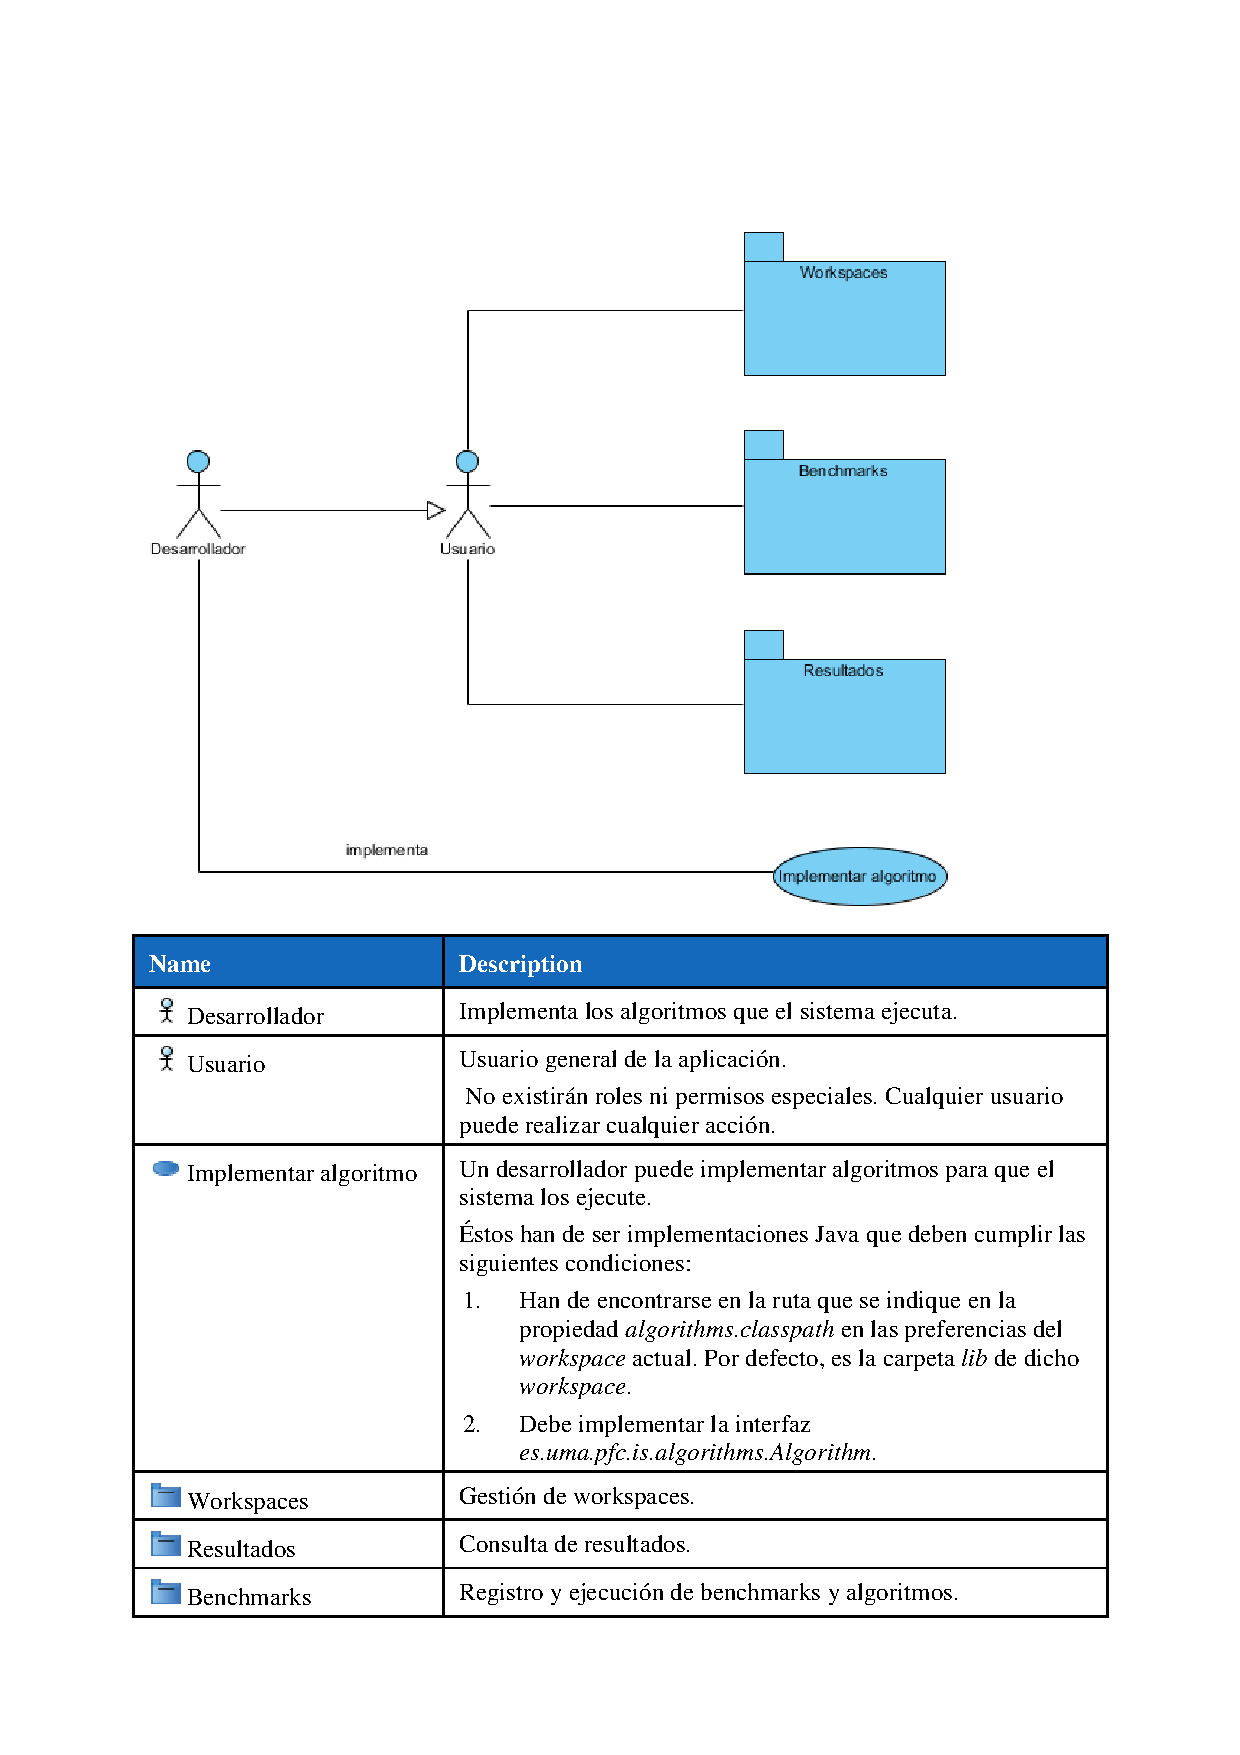
\includepdf[pages=-,pagecommand={}]{ext/cu_inicio.pdf}	
		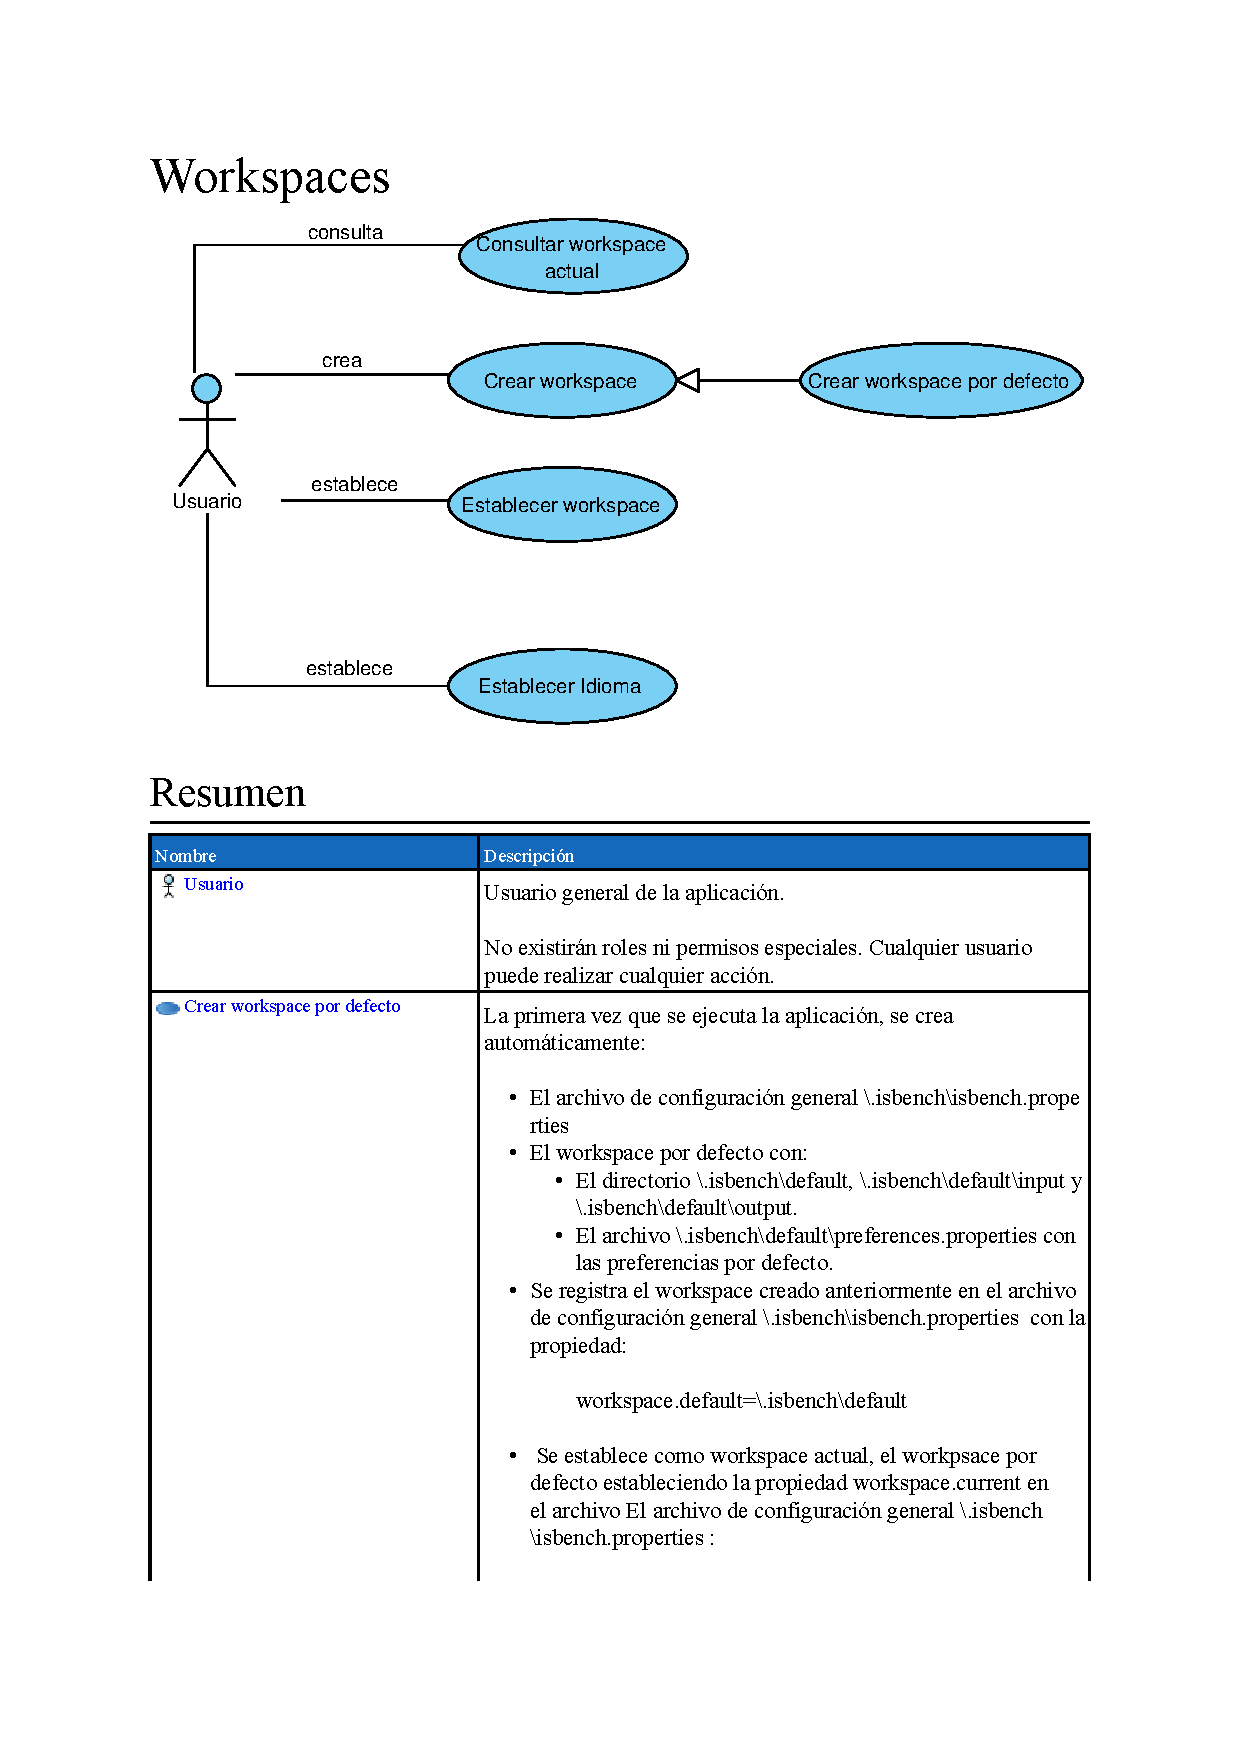
\includepdf[pages=-,pagecommand={}]{ext/cu_workspaces.pdf}
		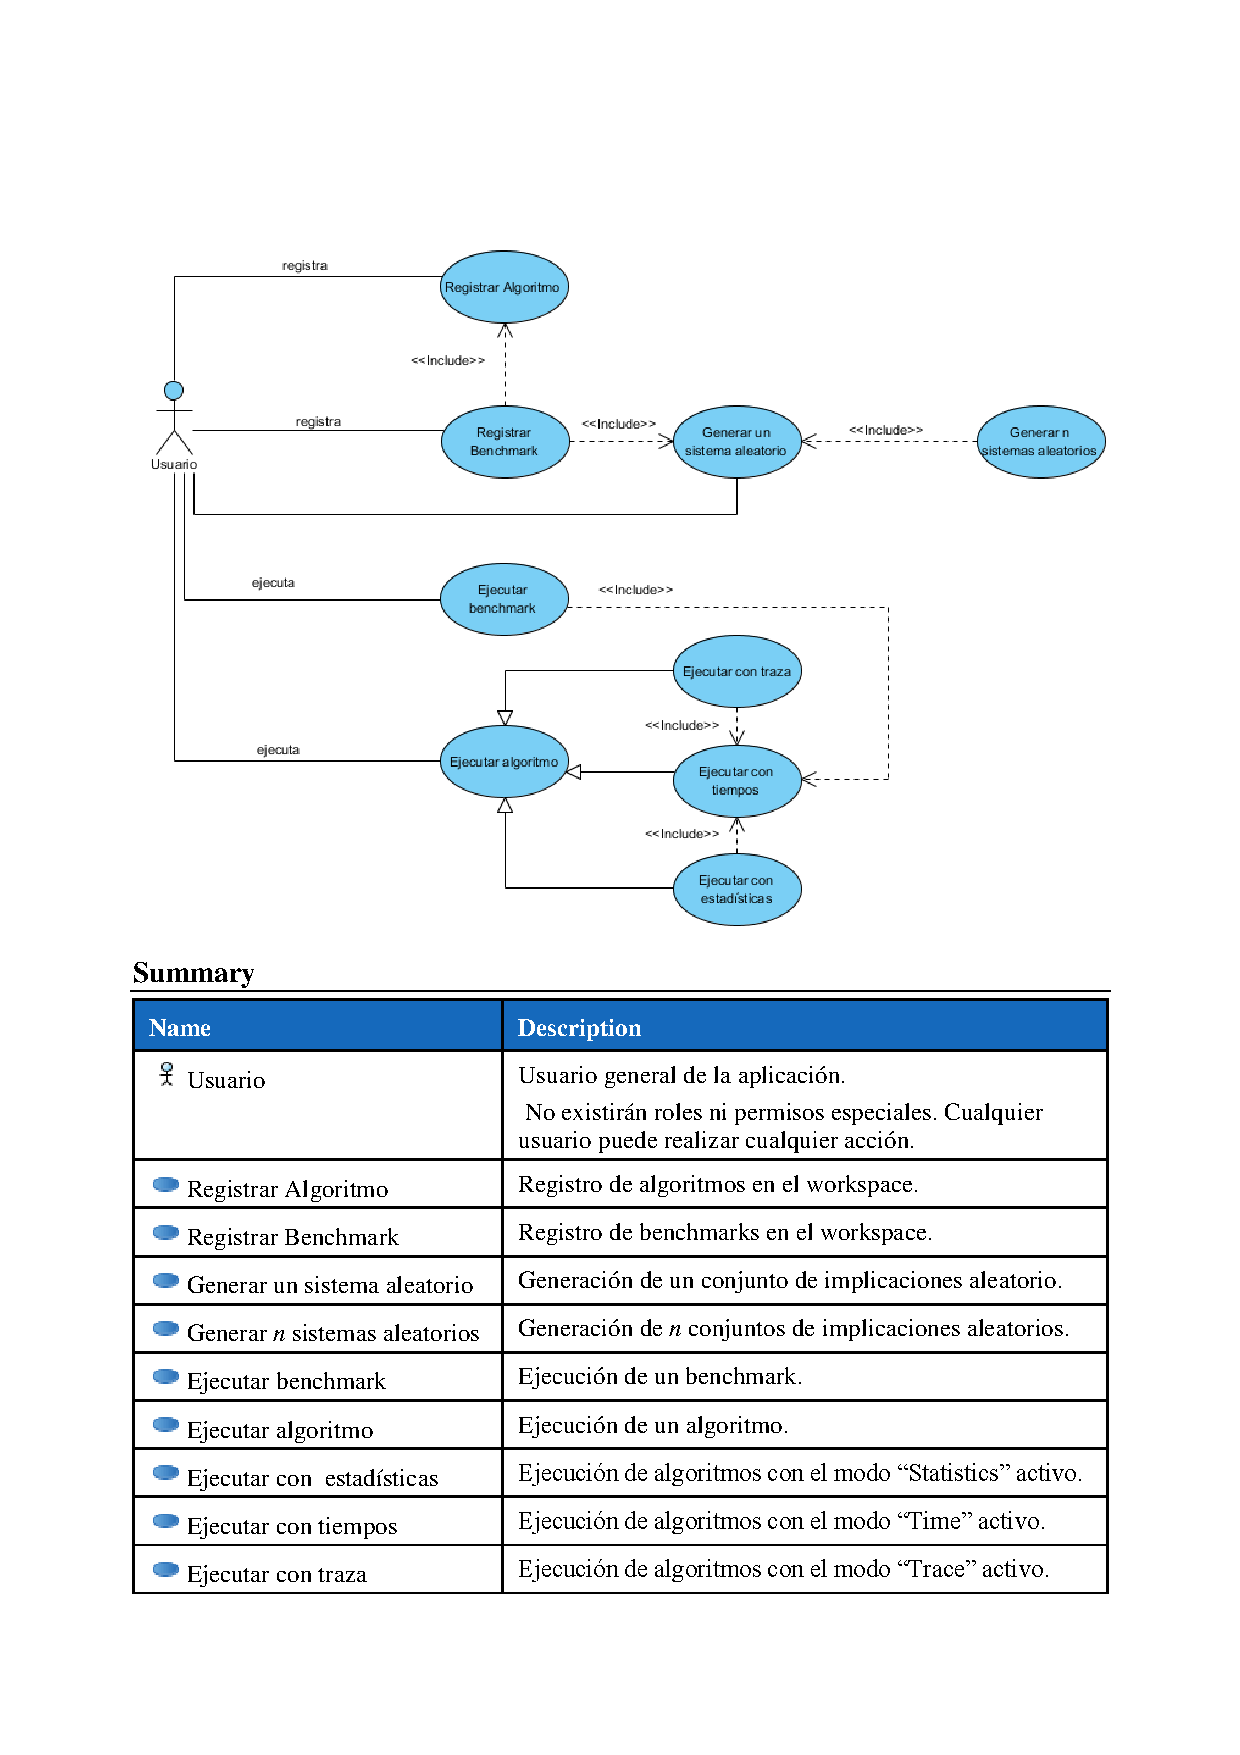
\includepdf[pages=-,pagecommand={}]{ext/cu_benchmarks.pdf}
		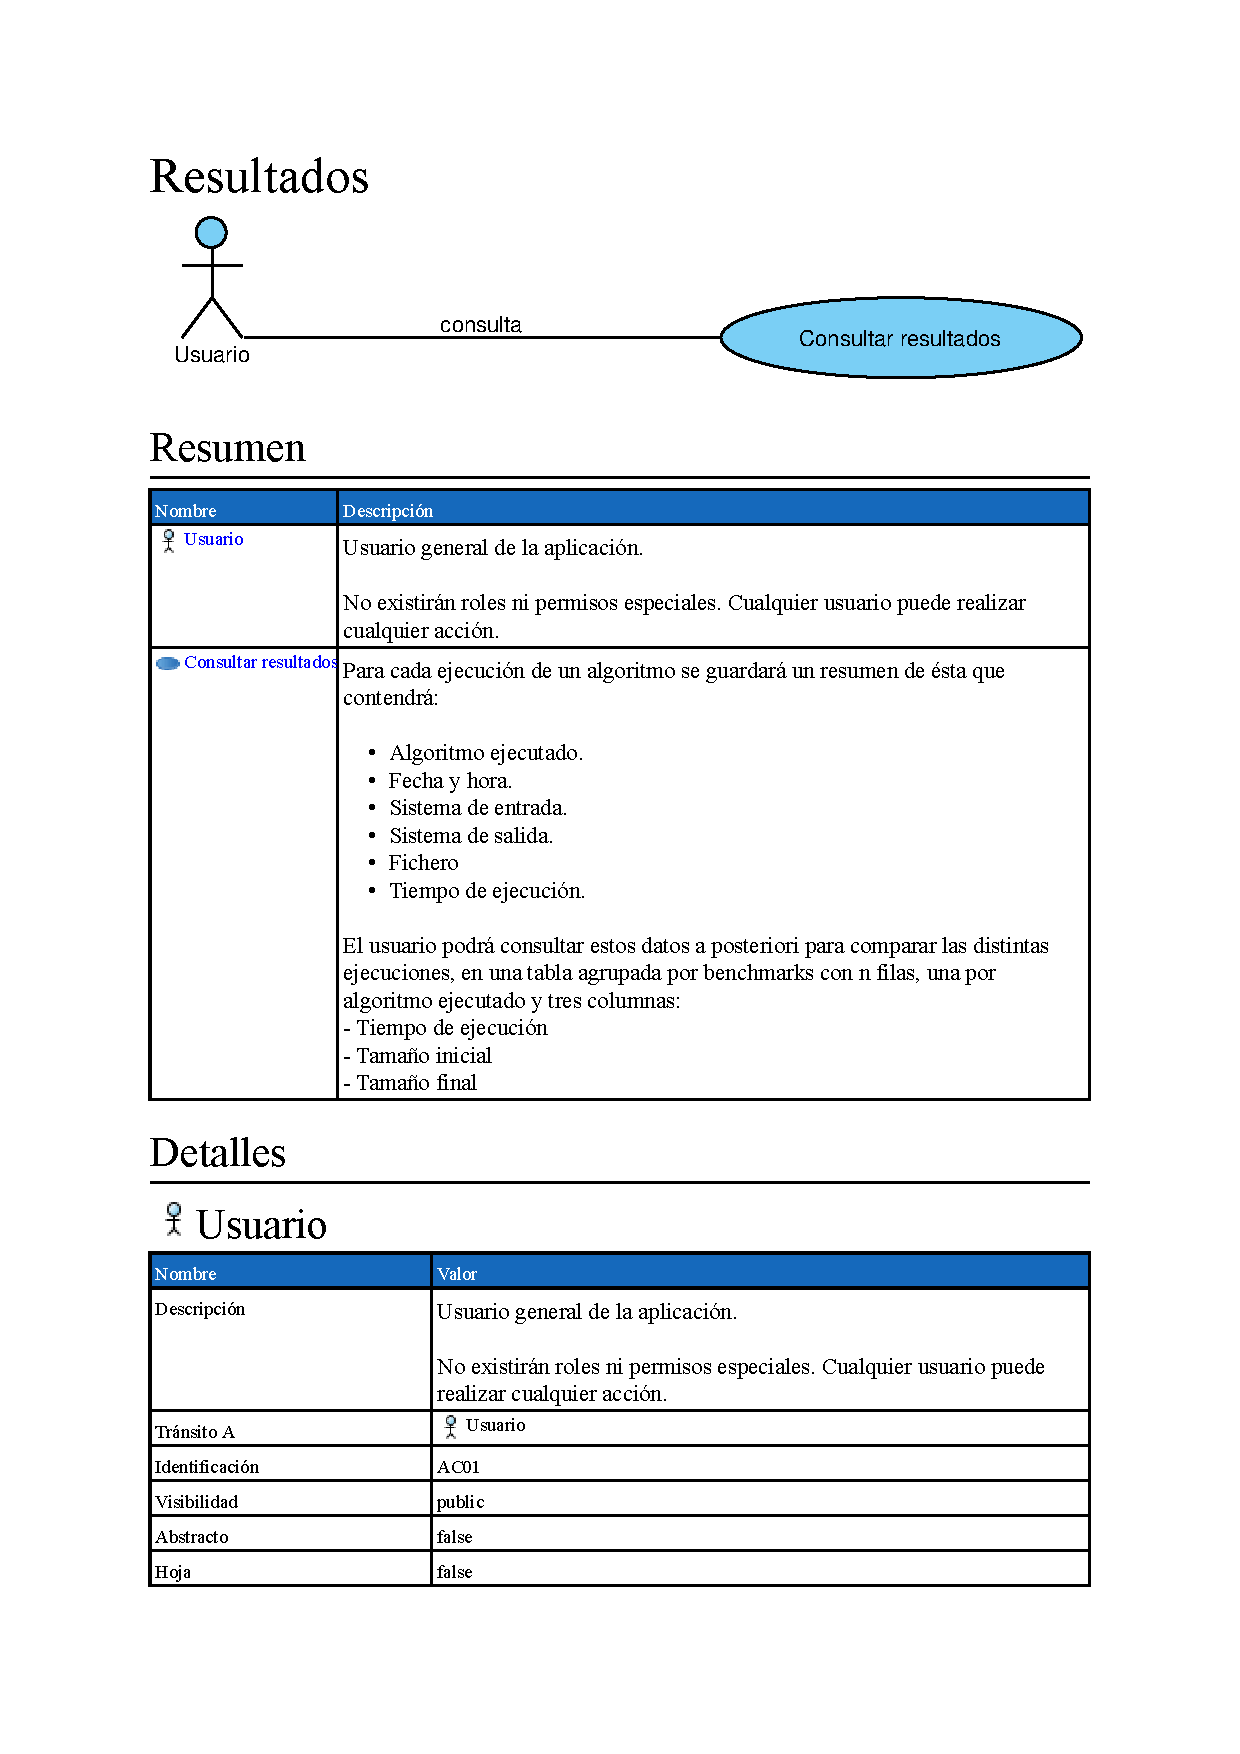
\includepdf[pages=-,pagecommand={}]{ext/cu_resultados.pdf}

\end{document}